\documentclass[margin=5mm]{standalone}
\usepackage[dvipsnames]{xcolor}
\usepackage{pgfplots}
\usepackage{tikz}
\usepackage[tikz]{ocgx2}

\pgfplotsset{compat=1.18}
\begin{document}

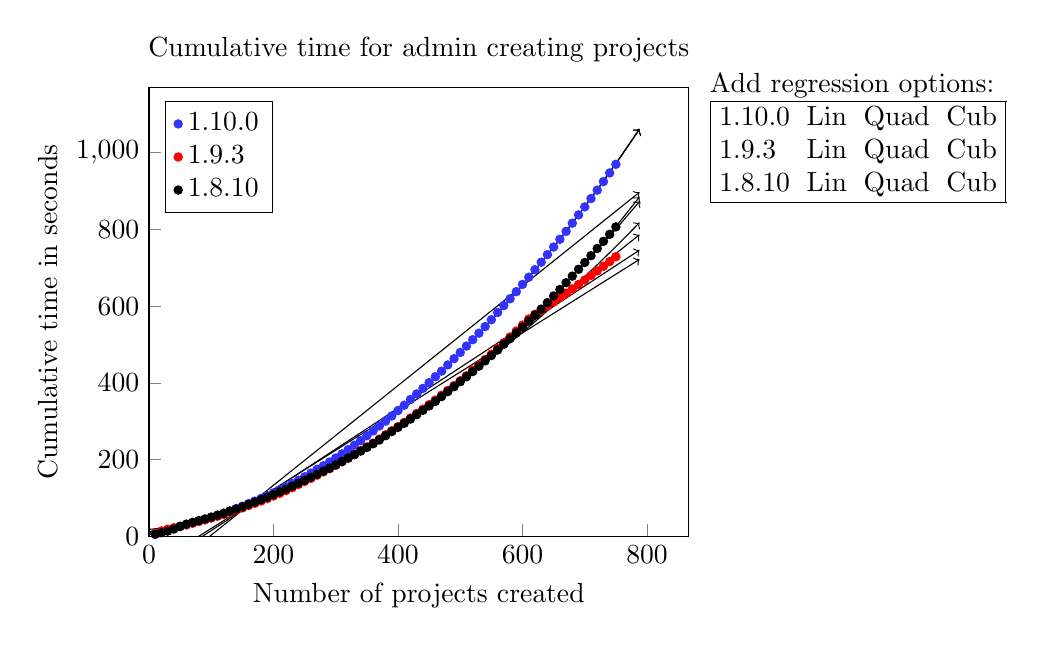
\begin{tikzpicture}
    \begin{axis}[
        align = center,
        legend pos = north west,
        legend cell align = left,
        xlabel = Number of projects created,
        ylabel = Cumulative time in seconds,
        xtick pos = left,
        ytick pos = left,
        scaled ticks = false,
        xmin = 0,
        ymin = 0,
        title = {Cumulative time for admin creating projects},
        title style = {text width = 0.8\textwidth},
        legend entries={\switchocg{1.10.0}{1.10.0},\switchocg{1.9.3}{1.9.3},\switchocg{1.8.10}{1.8.10}}]
        \begin{scope}[ocg = {ref = 1.10.0-Lin, status = invisible}]
            \plot[domain=0:788,->,forget plot] (\x,{-127.1262814414416197905666194856166839599609375 + 1.29991807396870573398928172537125647068023681640625*(\x)^1});
        \end{scope}
        \begin{scope}[ocg = {ref = 1.10.0-Quad, status = invisible}]
            \plot[domain=0:788,->,forget plot] (\x,{8.039748744908930433439309126697480678558349609375 + 0.2466762803088311528654230642132461071014404296875*(\x)^1 + 0.00138584446534194077015056389967639915994368493556976318359375*(\x)^2});
        \end{scope}
        \begin{scope}[ocg = {ref = 1.10.0-Cub, status = invisible}]
            \plot[domain=0:788,->,forget plot] (\x,{9.49655780081403833037256845273077487945556640625 + 0.2244080920390717770462885027882293798029422760009765625*(\x)^1 + 0.00145861215045208695954837008201820935937575995922088623046875*(\x)^2 + -0.000000063831302728198295749813414266815581044056671089492738246917724609375*(\x)^3});
        \end{scope}
        \begin{scope}[ocg = {ref = 1.10.0, status = visible}]
            \addplot[
                only marks,
                color = blue!80!white,
                mark = *,
                mark size = 1.5 pt
            ]coordinates {(10,5.523)(20,10.171)(30,15.265)(40,20.197)(50,25.084)(60,29.495)(70,34.057)(80,38.792)(90,43.585)(100,48.575)(110,53.829)(120,59.76)(130,65.719)(140,71.958)(150,78.168)(160,84.839)(170,91.453)(180,98.424)(190,105.337)(200,113.171)(210,120.999)(220,129.151)(230,137.419)(240,146.066)(250,154.842)(260,164.507)(270,174.235)(280,183.571)(290,193.432)(300,203.901)(310,214.615)(320,225.82)(330,237.344)(340,249.14)(350,262.037)(360,274.468)(370,287.427)(380,300.105)(390,313.517)(400,327.645)(410,341.539)(420,356.518)(430,371.061)(440,385.545)(450,400.405)(460,415.766)(470,430.48)(480,446.722)(490,463.118)(500,479.241)(510,495.934)(520,512.484)(530,529.443)(540,546.809)(550,564.586)(560,583.389)(570,601.415)(580,619.167)(590,637.727)(600,656.708)(610,675.42)(620,694.931)(630,714.62)(640,734.361)(650,754.172)(660,774.403)(670,795.084)(680,816.466)(690,838.021)(700,858.815)(710,880.665)(720,902.463)(730,924.748)(740,947.359)(750,969.966)};
        \end{scope}
        \begin{scope}[ocg = {ref = 1.9.3-Lin, status = invisible}]
            \plot[domain=0:788,->,forget plot] (\x,{-81.7901628828828251016602735035121440887451171875 + 1.0201276216216215164678260407526977360248565673828125*(\x)^1});
        \end{scope}
        \begin{scope}[ocg = {ref = 1.9.3-Quad, status = invisible}]
            \plot[domain=0:788,->,forget plot] (\x,{-3.65263335061086191757340202457271516323089599609375 + 0.411263755136385356081518693827092647552490234375*(\x)^1 + 0.000801136666427942488628854977861237784964032471179962158203125*(\x)^2});
        \end{scope}
        \begin{scope}[ocg = {ref = 1.9.3-Cub, status = invisible}]
            \plot[domain=0:788,->,forget plot] (\x,{17.7909744827017419765979866497218608856201171875 + 0.08348552333619106702311540857408544979989528656005859375*(\x)^1 + 0.001872245948811196956940161584270754246972501277923583984375*(\x)^2 + -0.000000939569545950223615328011743386138476807900588028132915496826171875*(\x)^3});
        \end{scope}
        \begin{scope}[ocg = {ref = 1.9.3, status = visible}]
            \addplot[
                only marks,
                color = red,
                mark = *,
                mark size = 1.5 pt
            ]coordinates {(10,6.107)(20,13.72)(30,18.13)(40,21.963)(50,25.848)(60,29.774)(70,34.103)(80,38.387)(90,42.578)(100,47.357)(110,52.091)(120,56.804)(130,62.428)(140,68.073)(150,73.776)(160,80.083)(170,85.822)(180,91.747)(190,98.192)(200,104.798)(210,111.843)(220,118.889)(230,126.481)(240,134.989)(250,142.814)(260,150.871)(270,159.254)(280,167.519)(290,175.935)(300,184.815)(310,194.147)(320,203.521)(330,212.978)(340,222.892)(350,232.662)(360,242.462)(370,253.451)(380,264.337)(390,274.915)(400,285.503)(410,296.738)(420,308.194)(430,320.059)(440,331.146)(450,343.026)(460,355.162)(470,367.734)(480,380.349)(490,392.79)(500,405.582)(510,418.542)(520,433.248)(530,446.958)(540,460.91)(550,474.696)(560,489.938)(570,504.622)(580,519.593)(590,535.143)(600,550.61)(610,566.547)(620,578.721)(630,589.228)(640,600.028)(650,611.289)(660,622.334)(670,633.712)(680,644.891)(690,656.293)(700,668.102)(710,680.008)(720,691.898)(730,704.057)(740,716.208)(750,728.96)};
        \end{scope}
        \begin{scope}[ocg = {ref = 1.8.10-Lin, status = invisible}]
            \plot[domain=0:788,->,forget plot] (\x,{-91.743610810810736211351468227803707122802734375 + 1.0633443442389758359922780073247849941253662109375*(\x)^1});
        \end{scope}
        \begin{scope}[ocg = {ref = 1.8.10-Quad, status = invisible}]
            \plot[domain=0:788,->,forget plot] (\x,{11.7312492410218585092707144212909042835235595703125 + 0.25704673344547490643208220717497169971466064453125*(\x)^1 + 0.001060917908938817204311799713423170032911002635955810546875*(\x)^2});
        \end{scope}
        \begin{scope}[ocg = {ref = 1.8.10-Cub, status = invisible}]
            \plot[domain=0:788,->,forget plot] (\x,{3.759612549261669212086189872934482991695404052734375 + 0.37889791631030600438378996841493062674999237060546875*(\x)^1 + 0.000662734258001743234585412256620884363655932247638702392578125*(\x)^2 + 0.000000349283904330766831064785001015327026152590406127274036407470703125*(\x)^3});
        \end{scope}
        \begin{scope}[ocg = {ref = 1.8.10, status = visible}]
            \addplot[
                only marks,
                color = black,
                mark = *,
                mark size = 1.5 pt
            ]coordinates {(10,4.997)(20,9.129)(30,13.252)(40,18.696)(50,25.699)(60,31.543)(70,35.964)(80,40.657)(90,44.934)(100,49.918)(110,54.907)(120,59.834)(130,65.357)(140,70.79)(150,76.454)(160,83.122)(170,89.072)(180,95.245)(190,101.922)(200,108.545)(210,115.543)(220,123.019)(230,130.152)(240,138.177)(250,145.788)(260,153.519)(270,161.443)(280,169.54)(290,177.473)(300,185.945)(310,194.626)(320,203.858)(330,212.741)(340,221.998)(350,231.427)(360,241.202)(370,250.893)(380,262.064)(390,272.973)(400,283.713)(410,294.529)(420,305.546)(430,316.936)(440,328.372)(450,339.841)(460,351.644)(470,364.177)(480,377.185)(490,389.924)(500,402.797)(510,415.93)(520,429.354)(530,443.51)(540,457.3)(550,471.119)(560,485.59)(570,500.611)(580,515.254)(590,529.987)(600,545.284)(610,561.081)(620,576.753)(630,592.36)(640,609.055)(650,626.503)(660,643.495)(670,661.092)(680,678.268)(690,696.127)(700,713.805)(710,731.587)(720,750.371)(730,768.929)(740,787.393)(750,806.703)};
        \end{scope}
    \end{axis}
    \begin{scope}
        \addtolength{\tabcolsep}{-0.3em}
        \node [below right, shape=rectangle, align=left](regressiontable) at (7,6) {
            Add regression options: \\
            \begin{tabular}{|llll|}
                \hline
                1.10.0 & \switchocg{1.10.0-Lin}{Lin} & \switchocg{1.10.0-Quad}{Quad} & \switchocg{1.10.0-Cub}{Cub} \\
                1.9.3 & \switchocg{1.9.3-Lin}{Lin} & \switchocg{1.9.3-Quad}{Quad} & \switchocg{1.9.3-Cub}{Cub} \\
                1.8.10 & \switchocg{1.8.10-Lin}{Lin} & \switchocg{1.8.10-Quad}{Quad} & \switchocg{1.8.10-Cub}{Cub} \\
                \hline
            \end{tabular}
        };
    \end{scope}
\end{tikzpicture}

\end{document}